\begin{frame}{collision detection}
    \begin{itemize}
    \item Wi-Fi: use ACKs to detect if transmission successful
    \item problem: transmit whole packet, then know about collision
    \vspace{.5cm}
    \item alternate idea: listen for collision, stop transmitting early
    \item doesn't work on wireless (we'll talk about why later)
    \item but does work on some wired shared media
    \item part of reason for design of Ethernet header
    \end{itemize}
\end{frame}

\usetikzlibrary{arrows.meta,shapes,shapes.misc}
\begin{frame}{collision detection takes time}
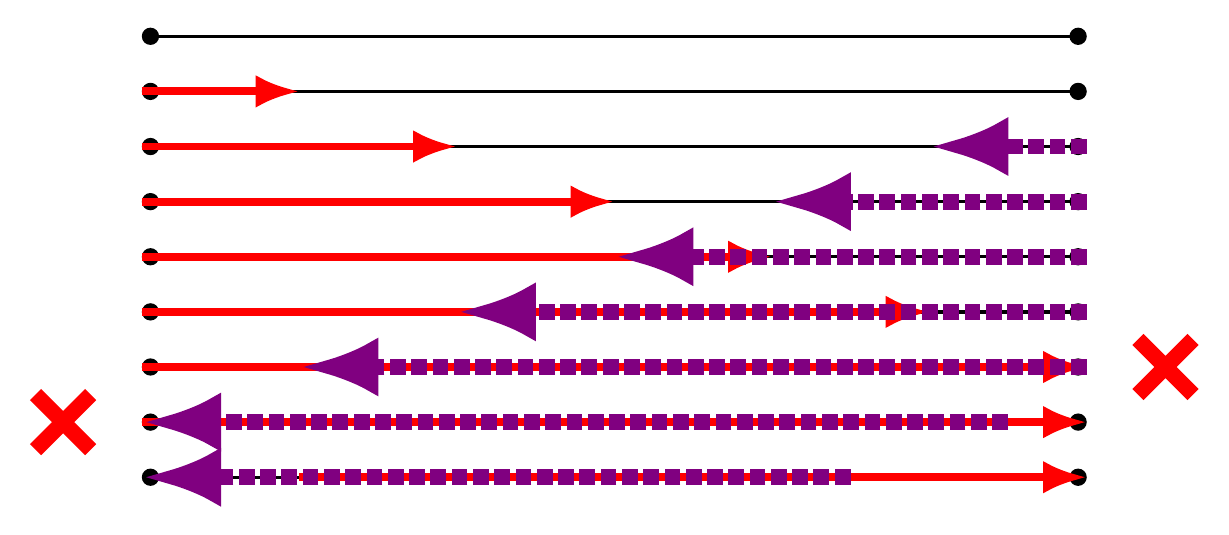
\begin{tikzpicture}[y=0.7cm]
\tikzset{
    wire/.style={draw,very thick,Circle-Circle},
    signal1/.style={draw,line width=1mm,red,-Latex},
    signal2/.style={draw,line width=2mm,dotted,violet,-Latex},
}
\draw[wire] (0, 0) -- (12, 0);
\draw[wire] (0, -1) -- (12, -1);
\draw[signal1] (0, -1) -- (2, -1);

\draw[wire] (0, -2) -- (12, -2);
\draw[signal1] (0, -2) -- (4, -2);
\draw[signal2] (12, -2) -- (10, -2);

\draw[wire] (0, -3) -- (12, -3);
\draw[signal1] (0, -3) -- (6, -3);
\draw[signal2] (12, -3) -- (8, -3);

\draw[wire] (0, -4) -- (12, -4);
\draw[signal1] (0, -4) -- (8, -4);
\draw[signal2] (12, -4) -- (6, -4);

\draw[wire] (0, -5) -- (12, -5);
\draw[signal1] (0, -5) -- (10, -5);
\draw[signal2] (12, -5) -- (4, -5);

\draw[wire] (0, -6) -- (12, -6);
\draw[signal1] (0, -6) -- (12, -6);
\draw[signal2] (12, -6) -- (2, -6);
\node[draw=red,line width=2mm,minimum width=.5cm,minimum height=.5cm,cross out] at (13, -6) {};

\draw[wire] (0, -7) -- (12, -7);
\draw[signal1] (0, -7) -- (12, -7);
\draw[signal2] (11, -7) -- (0, -7);
\node[draw=red,line width=2mm,minimum width=.5cm,minimum height=.5cm,cross out] at (-1, -7) {};

\draw[wire] (0, -8) -- (12, -8);
\draw[signal1] (2, -8) -- (12, -8);
\draw[signal2] (9, -8) -- (0, -8);
\end{tikzpicture}
\end{frame}

\begin{frame}{exercise: Ethernet cable length/delay}
    \begin{itemize}
    \item copper cable: about 2/3rds speed of light propogation
    \item 100Mbit ethernet has 64byte minimum frame size
    \vspace{.5cm}
    \item exercise: maximum cable length with collision detection?
    \end{itemize}
\end{frame}

\begin{frame}{solution}
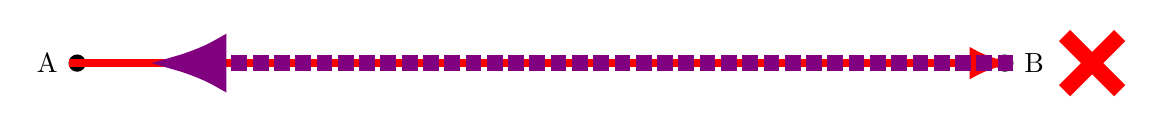
\begin{tikzpicture}[y=0.7cm]
\tikzset{
    wire/.style={draw,very thick,Circle-Circle},
    signal1/.style={draw,line width=1mm,red,-Latex},
    signal2/.style={draw,line width=2mm,dotted,violet,-Latex},
}
\draw[wire] (0, -6) node[left]{A} -- (12, -6) node[right] {B};
\draw[signal1] (0, -6) -- (12, -6);
\draw[signal2] (12, -6) -- (1, -6);
\node[draw=red,line width=2mm,minimum width=.5cm,minimum height=.5cm,cross out] at (13, -6) {};
\end{tikzpicture}
\begin{itemize}
\item A and B maximally far apart on network and collide
    \begin{itemize}
    \item need them to detect collision and resend
    \item if they're maximum distance, then anyone else will get interference
    \end{itemize}
\item A transmits at time 0, takes $X$ time units to reach B
\item B transmits at time $X-\epsilon$, then detects collision
\item need A to also detect collision before it finishes sending frame
\item maximum packet length is how much we can send in $2X$ time units
\item 2X = 64 times 8 / 100Mbps  = 5.12 $\mu$ s; X = 2.56 $\mu$s
\end{itemize}
\end{frame}

\begin{frame}{propogation delay}
\begin{itemize}
\item transmission time for 64 bytes is 2.56 $\mu$s
\item propogation delay: approx 0.2 meters/ns or 200 meters/$\mu$s
\item 2.56 $\mu$s is about 512 meteres
\end{itemize}
\end{frame}


\begin{frame}{exercise: 802.11b distance}
    \begin{itemize}
    \item 50 $\mu s$ minimum interframe spacing
    \item 10 $\mu s$ slots after that if contention
    \item speed of light propogation
    \item need to detect channel quiet this time minimum before transmitting
    \item 11Mbps max bitrate; $\sim$288 minimum frame size
    \vspace{.5cm}
    \item exercise: 50 $\mu s$ includes time for ACK --- maximum distance before too little?
    \item exercise: what distance before carrier sense not useful?
    \end{itemize}
\end{frame}

\begin{frame}{}
\begin{itemize}
\item 50 microsecond around 15000 metres
\item 10 microsecond means signal goes approx. 3000 metres
    \begin{itemize}
    \item distance where we won't detect transmission in previous slot accurately
    \item one way for carrier sense not to be very useful
    \end{itemize}
\item 288/11 approx. 27 microsec 
\item have 50 microsecond to detect transmission
    \begin{itemize}
    \item gives around 23 microsec propogation delay $\sim$ 8000 metres
    \end{itemize}
\end{itemize}
\end{frame}
